\section{Data Race Detection} \label{sec:drd}
A Computation Graph for a task parallel program is a directed acyclic graph that represents the execution of the program \cite{dennis2012determinacy}. It is modified here to track memory locations accessed by tasks. 

\begin{definition}
\textbf{Computation Graph:} A Computation Graph 
$G = \tuple{N, E, \delta, \omega}$ of a task parallel program \textbf{P} with input $\psi$ is a directed acyclic graph where $N$ is a finite set of nodes, $E \subseteq N \times N$ is a set of directed edges, $\delta$ is the function that maps $N$ to the unique identifiers for the shared locations read by the tasks: $\delta : (N \mapsto 2^{V})$, $\omega$ is the function that maps $N$ to the unique identifiers for the shared locations written by the tasks: $\omega : (N \mapsto 2^{V})$, and V is the set of the unique identifiers for the shared locations.
\end{definition}



\begin{figure}
  \centering
        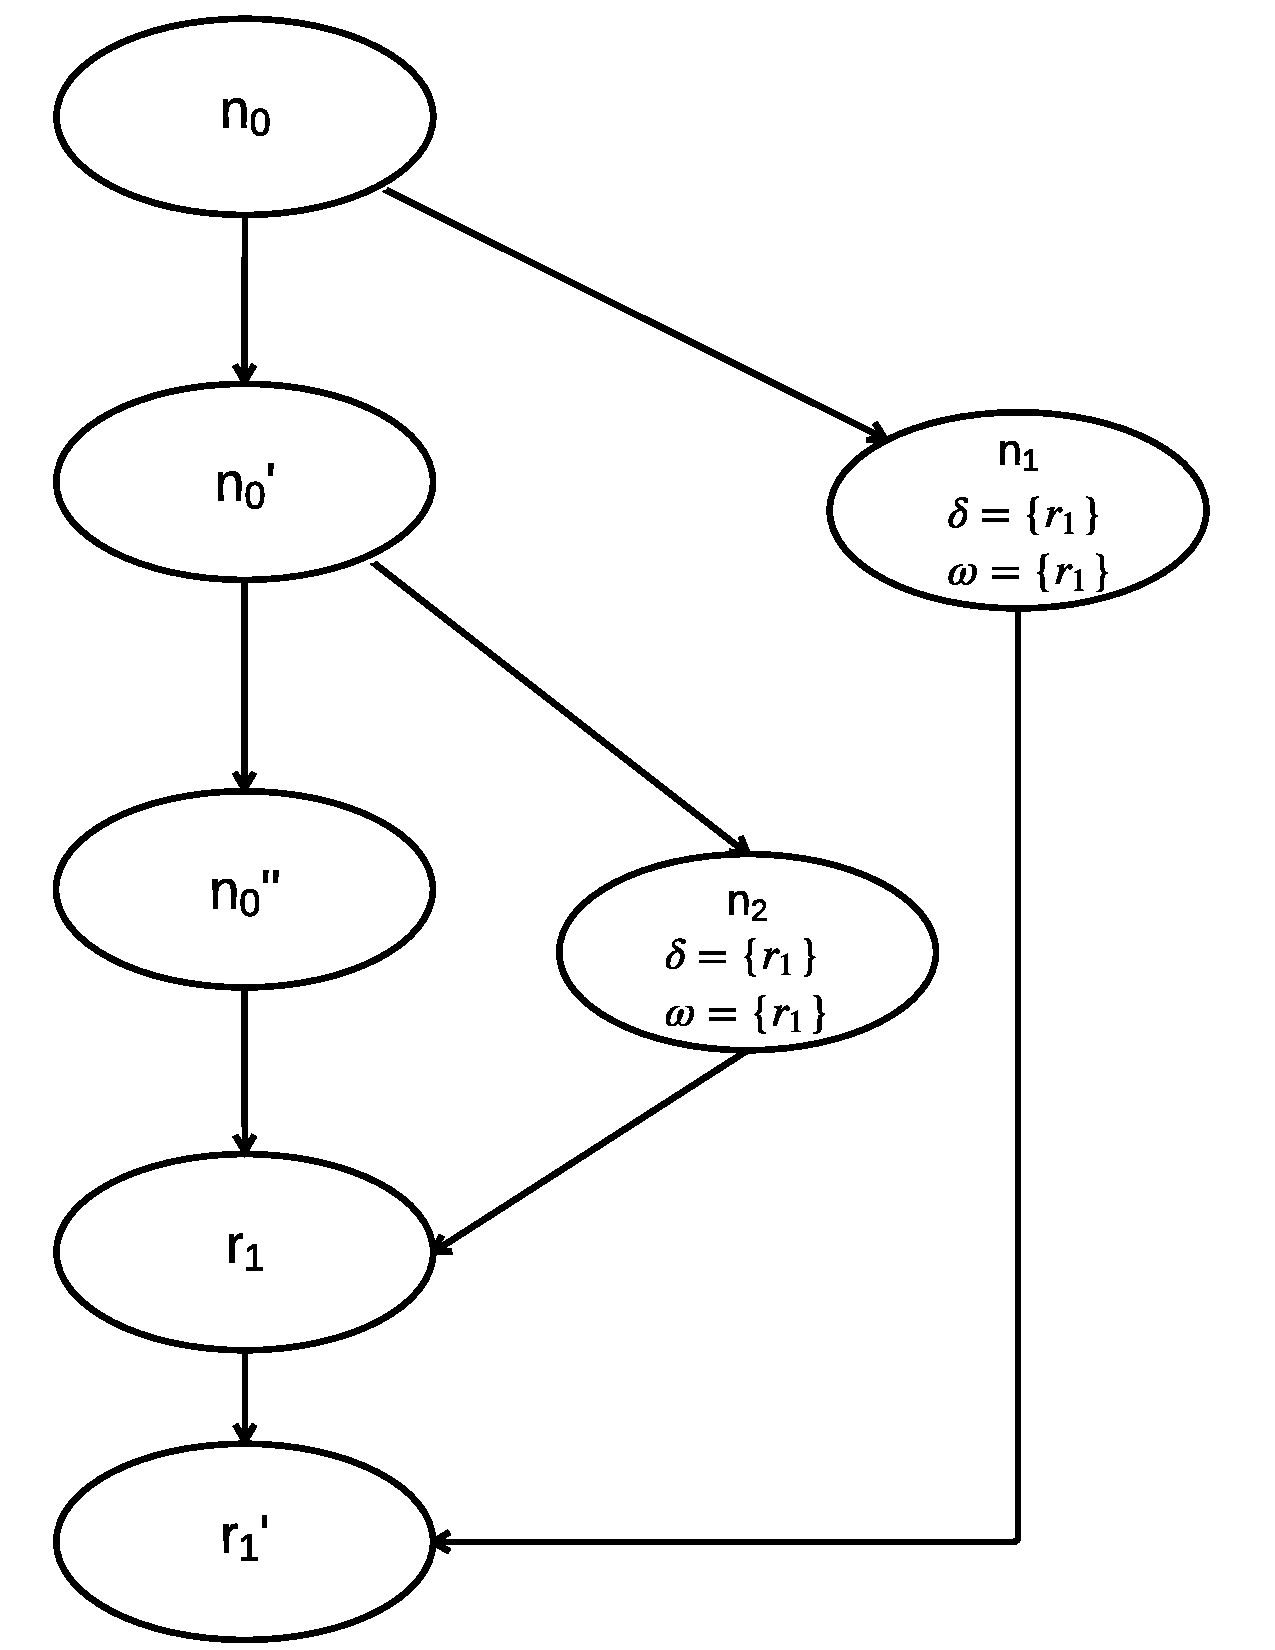
\includegraphics[width=0.3\textwidth]{../figs/Fig3-1.pdf}
    \caption{Computation Graph Example.}
    \label{fig:cg}
    \vspace{-1em}
\end{figure}

\figref{fig:cg} is simple computation graph with nodes. Every node represents a block of sequential operations and edges order the nodes. The order between any two nodes $n_1$ and $n_2$ is given as $n_1 \prec n_2$, meaning that $n_1$ happens before $n_2$. Parallel nodes are un-ordered: $n_1 \nprec n_2$ and $n_2 \nprec n_1$. Data-race detection finds un-ordered nodes with conflicting accesses. For the example, nodes $n_1$ and $n_2$ are unordered and both are writing to variable $r_1$.

\begin{algorithm}[t]
  \caption{Data Race detection in a computation graph } \label{algo:drd}
\begin{algorithmic}[1]
\Function{DetectRace}{$Computation Graph \ G$}
\State N := Topologically ordered nodes in G \label{loc:topo}
\For {i in [1, $|N|$]}
\State $n = N[i]$
\For {j in [i+1, $|N|$]} 
\State $n' := N[j]$
\If {$ (n \nprec n') $}  \label{loc:path} \label{loc:forall}
		\If {$((\delta(n) \cap \omega(n') \neq \emptyset)  \lor  (\omega(n) \cap \delta(n') \neq \emptyset) \lor (\omega(n) \cap \omega(n') \neq \emptyset) )$} \label{loc:intersection}
			\State \textbf{Report Data Race and Exit} \label{loc:datarace}
		\EndIf
\EndIf
 \EndFor
 \EndFor
\EndFunction  
\end{algorithmic}
\end{algorithm}

A naive approach to data-race detection given a computation graph is in \algoref{algo:drd}. The nodes in the computation graph are added to a topologically sorted set on \lineref{loc:topo}. The $i^{th}$ node in the set is given by $N[i]$. The nodes are traversed in order and each node is compared to every node that comes later in the topological ordering. \lineref{loc:path} checks if the nodes $n$ and $n'$ are un-ordered. If the nodes are un-ordered, then the sets of memory locations accessed by each node are checked for conflict on \lineref{loc:intersection}. If any of the sets shares an element, then there is a data race.

The algorithm is purposely naive and can be improved if needed \cite{mellor1991fly,raman2012scalable}; though, it is not the goal of the research presented here because problem instances are assumed to be small enough for model checking which is limited by the number of computation graphs that must be enumerated rather than the size of those graphs.

\begin{comment}
: $\mathcal{O}$(N$^2$). When nodes are topologically ordered, reachability of nodes can be checked in $\mathcal{O}$(N) time. Therefore, the time required to check if two nodes are executing in parallel is $\mathcal{O}$(N$^2$). The time required to check the intersection of read or write sets of shared locations is $\mathcal{O}$($m_1 +  m_2$) where $m_1$ and $m_2$ are the sizes of the two sets. ($m_1 + m_2$) is much smaller than N. Therefore, the time complexity of Algorithm \ref{algo:drd}  is $\mathcal{O}$(N$^2$).
\end{comment}

\begin{comment}
A data race detection algorithm is sound if it does not miss any data race in a program for a given input (e.g., it may under-approximate the set of data race free programs), and it is complete if it does not report data races in programs that are data race free (e.g., it may over-approximate the set of data race free programs.
\end{comment}

\begin{theorem} \label{thm:graph}
Using the tree semantics with Algorithm \ref{algo:drd} to detect data-race in the resulting computation graph is complete for a task parallel program with a given input.
\end{theorem}

\begin{comment}
\begin{proof}
The computation graph is a directed acyclic graph. The transitive closure of the graph gives the reachibility relationship of the tasks. The transitive closure is a strict partial order over the nodes of the graph. The data race detection algorithm checks if nodes $n$ and $n^\prime$ in the graph are unordered on Line \ref{loc:forall}. The statements may be executed in parallel by these nodes. The memory accessed by these tasks is compared and a race is reported if a conflict is detected on Line \ref{loc:datarace}. Therefore, when algorithm \ref{algo:drd} declares a computation graph to be data race free, no race can exist in that graph and when a race is reported by the algorithm, there definitely exists two tasks that execute in parallel and have conflicting accesses to a shared variable. Hence, Algorithm \ref{algo:drd} is sound and complete for a given computation graph.
\end{proof}
\end{comment}
